\cleardoublepage

\chapter{Exploración del modelo predictivo}
\label{makereference4}

\section{Introducción a los modelos predictivos}
\label{makereference4.1}

Cuando hablamos de \textbf{modelos predictivos} nos estamos refiriendo al análisis que agrupa una serie de técnicas para conseguir \textbf{analizar datos reales} tanto actuales como históricos y así conseguir \textbf{predicciones}. Con esta predicción podremos saber cuánto se acerca nuestra predicción a la realidad.

Existen algunos conceptos clave a la hora de hablar de metodos predictivos:

\begin{itemize}
	\item \textbf{Conjunto de entrenamiento:} son los datos que se utiliza para desarrollar los modelos predictivos.
	\item \textbf{Conjunto de validación:} conjunto de datos utilizados para evaluar el rendimiento de dichos modelos.
	\item \textbf{Predictores:} variables de entrada, utilizadas para la ecuación de predicción. 
	\item \textbf{Resultado:} objetivo que se quiere predecir.
\end{itemize}

Las fases para desarrollar este tipo de modelos son las siguientes:
\begin{itemize}
\item \textbf{Entrenamiento:} se selecciona un conjunto de datos (\textbf{conjunto de entrenamiento}) del que se conoce el valor real de la predicción que queremos realizar y se explora, en función del algoritmo seleccionado, para obtener un posible modelo.

Cada modelo tiene una serie de variables que podemos definir previas al entrenamiento que influirán en el resultado. En esta fase, los factores que se buscan explorar son aquellos que, internamente, ajusta el propio algoritmo en función de los datos de entrada y los parámetros de entrada que definamos.

\item \textbf{Validación:} se selecciona otro conjunto de datos distinto al anterior (\textbf{conjunto de validación}) del que también se conoce el valor real de la predicción y se aplica el modelo obtenido en el entrenamiento. Se comparan los datos proporcionados con el modelo con los datos reales y se sacan distintas métricas para conocer su efectividad. 

En función del resultado obtenido en la validación, se pueden volver a repetir estos dos pasos cambiando el conjunto de datos o los parámetros de entrada del modelo hasta conseguir una predicción óptima.

\item \textbf{Predicción:} una vez encontrado un modelo en la fase anterior que cumpla con los requisitos, se guarda ese modelo en algún formato recuperable para poder utilizarlo en cualquier momento sin tener que volver a entrenarlo.
\end{itemize}

Los algoritmos predictivos que se han estudiado han sido los siguientes:

	\begin{itemize}
	\item Regresión Lineal
	\item SVR (Support Vector Regression)
	\item Redes Neuronales
\end{itemize}

\section{Conjunto de datos}
\label{makereference4.2}

Para poder encontrar el modelo más adecuado para este problema se necesita una gran cantidad de datos con la que entrenar y validar. Estos datos han sido obtenidos de \href{http://www.inforiego.org/opencms/opencms}{InfoRiego}, una herramienta pensada para estudiar el consumo de agua en los cultivos y hacerlo más eficiente que proporciona la información meteorológica que necesaria para este proyecto.

\textbf{InfoRiego} hace uso de la red de estaciones meteorológicas SIAR (proyecto de la Dirección General de Desarrollo Rural del Ministerio de Medio Ambiente y Medio Rural y Marino) y de las estaciones del ITACyL (Instituto Tecnológico Agrario de Castilla y León).

Hay dos formas de obtener los datos de InfoRiego: a través de una API Rest o a través de FTP.

Este proyecto realiza la consulta de datos a través del servidor FTP de inforiego. Este servidor proporciona acceso mediante HTTP por lo que se obtienen los archivos con la información meteorológica deseada a través de \textbf{WebScrapping}.

\textbf{WebScrapping} es una técnica que recorre, a través de software, los elementos HTML de un sitio web pudiendo así obtener su información.

Se ha creado un script en Python que, dados unos parámetros de consulta (fecha y hora de inicio, fecha y hora de fin y ubicación) obtiene, a través de WebScrapping, los archivos CSV almacenados en InfoRiego que cumplen con los parámetros y los combina en un solo archivo CSV con toda la información. Ver figura \ref{inforiego}

\begin{figure}[htb]
	\begin{center}
		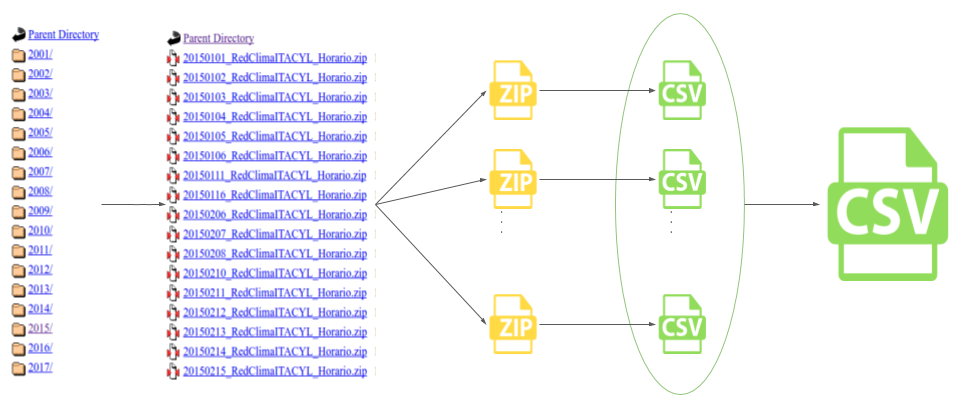
\includegraphics[width=15cm]{figures/inforiego.png}
		\caption{Flujo de obtención de datos de InfoRiego}
	\end{center}
	\label{inforiego}
\end{figure}

Este archivo CSV resultante (o el que se requiera en cada momento), es el utilizado como conjunto de entrenamiento y validación. La automatización de esta tarea permite que la exploración del modelo se pueda realizar de forma cómoda, pudiendo realizar así muchas más pruebas.

Los datos proporcionados a cualquier modelo predictivo son previamente \textbf{normalizados}. Es importante que todos estén en la misma escala ya que, de no ser así, se puede interpretar que los datos en una mayor escala tienen un mayor peso dentro de la predicción.

Para dicha normalización, son necesarios conocer el máximo, el mínimo y la media del conjunto de datos a normalizar. Estos datos serán almacenados para, posteriormente, poder invertir el proceso y obtener el valor inicial.

\begin{figure}[htb]
	\begin{center}
		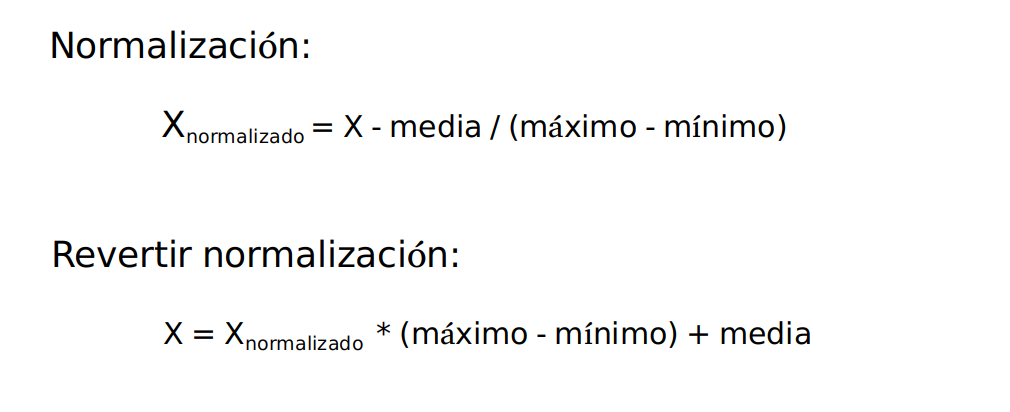
\includegraphics[width=15cm]{figures/normalizacion.png}
		\caption{Fórmulas de normalización}
	\end{center}
	\label{normalizacion}
\end{figure}

Este conjunto de datos debe sufrir una transformación más antes de poder ser utilizado en el entrenamiento. El entrenamiento y la validación necesitan dos elementos: los datos con los que se realiza la predicción y el resultado real que debe obtener. A estos dos elementos los llamaremos conjunto X y conjunto Y. Ver figura \ref{x_y}.

Ambos conjuntos parten del mismo conjunto de datos generado anteriormente.

El \textbf{conjunto X} tiene una serie de registros. Cada uno de ellos representa los datos necesarios para realizar una predicción. En este caso, son necesarias la \textbf{fecha}, \textbf{hora}, \textbf{temperatura}, \textbf{humedad} y \textbf{radiación} de varios instantes anteriores para realizar una predicción en un instante posterior.

El número de instantes anteriores lo llamaremos \textbf{k} por lo que serán necesarias las ``k'' muestras anteriores de hora, temperatura, humedad y radiación (la fecha y la ubicación serán la misma para todos los instantes anteriores). Indicando varios instantes anteriores indicamos que cada predicción se realiza con una ``tendencia'' que se espera que el algoritmo puede ser capáz de inferir.

Cada registro del \textbf{conjunto Y} indica la predicción que debe obtener cada registro en el mismo índice del \textbf{conjunto X}. Para obtener este valor, se recorre el conjunto X y se toma la radiación que ocurrió \textbf{n} instantes después en el conjunto de datos principal.

\begin{figure}[htb]
	\begin{center}
		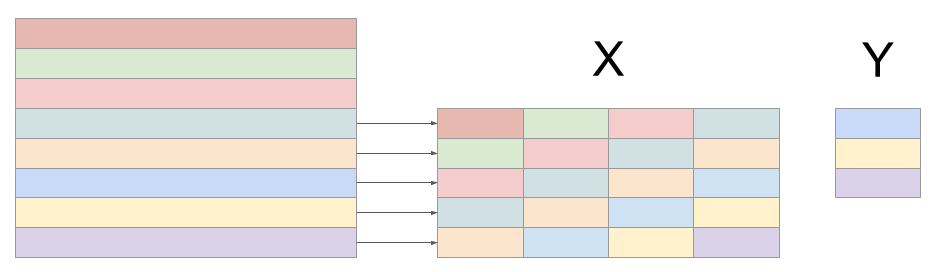
\includegraphics[width=14cm]{figures/datos_x_y.png}
		\caption{Transformación de datos para entrenamiento}
	\end{center}
	\label{x_y}
\end{figure}

\section{Algoritmos utilizados}
\label{makereference4.3}
	\subsection{Regresión Lineal}
	\label{makereference4.3.1}

	La \textbf{regresión lineal} es un modelo matemático que trata de hallar los coeficientes de una \textbf{combinación lineal} que mejor se ajusten a un conjunto de puntos dispersos conocidos a través del método de los \textbf{mínimos cuadrados}. Esto es, trazar una línea en el espacio que pase lo más próximo posible a todos los puntos.

	Al conocer dicha función lineal, podremos \textbf{``predecir''} con cierto grado de exactitud, lo que pasará.

	\begin{figure}[htb]
		\begin{center}
			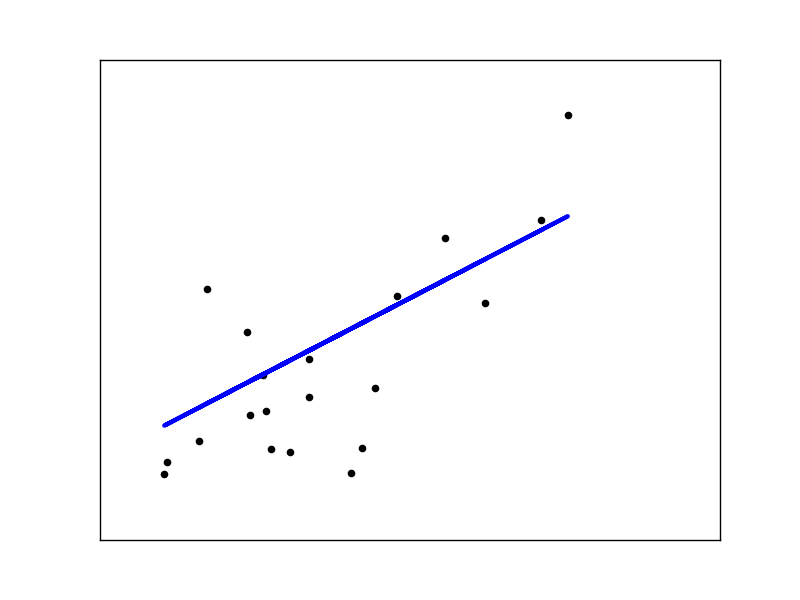
\includegraphics[height=3.5in]{figures/regression.png}
			\caption{Regresión lineal [Fuente: \href{www.wikipedia.org}{Wikipedia}]}
		\end{center}
		\label{regression}
	\end{figure}
	
	La recta que se puede ver en la gráfica \ref{regression}, muestra cómo la \textbf{regresión lineal} intenta dibujar una línea que minimice mejor la suma residual de cuadrados entre las respuestas observadas en el conjunto de datos, y las respuestas predichas por la aproximación lineal.
	También se calculan los coeficientes, la suma residual de cuadrados y el puntaje de varianza.

	\subsection{SVR (Support Vector Regression)}
	\label{makereference4.3.2}

	SRV es una nueva versión de SVM para regresión. SVM es un algoritmo de aprendizaje supervisado de la familia de los \textbf{clasificadores}.

	El término \textbf{clasificador} se utiliza en referencia al algoritmo utilizado para asignar un elemento entrante no etiquetado en una categoría concreta conocida. Dicho algoritmo, permite pues, ordenar o disponer por clases elementos entrantes, a partir de cierta información característica de estos.

	En SVM los datos son etiquetados en distintas clases y el clasificador intentará construir un hiperplano o conjunto de hiperplanos dentro del conjunto de datos que mejor separe las clases unas de otras. Ver figura \ref{svm}.

	\begin{figure}[htb]
		
		\begin{center}
			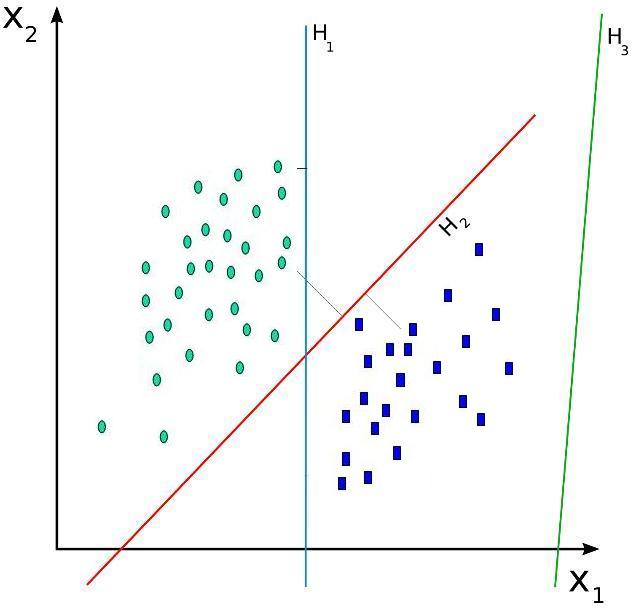
\includegraphics[height=3.5in]{figures/svm.jpg}
			\caption{SVM [Fuente: \href{www.wikipedia.org}{Wikipedia}]}
		\end{center}
		\label{svm}
	\end{figure}

	Las características más notables de los clasificadores SVM son:
	\begin{itemize}
		\item Proyectar previamente los datos a un espacio de dimensionalidad superior.
		\item Buscar el hiperplano que tenga la máxima distancia con los puntos que estén más cerca de él mismo. Es decir, que dejen una mayor margen entre los datos.
	\end{itemize}

	La diferencia entre SVR y SVM es que SVR intenta hacer una regresión a partir de el clasificador. Para esto, realiza un mapeo no lineal de los datos del entrenamiento a un espacio de mayor dimensión, donde podremos realizar una regresión lineal. Ver figura \ref{svr}.

	SVR permite varios modos de predicción ``kernel'': linear, poly, rbf, sigmoid...
	Este entrenamieto se ha llevado a cabo con los modos ``linear'' y ``rbf'' que, intuitivamente, pueden ser los que mas se acercan a nuestros datos reales.

	\begin{figure}[htb]
		\begin{center}
			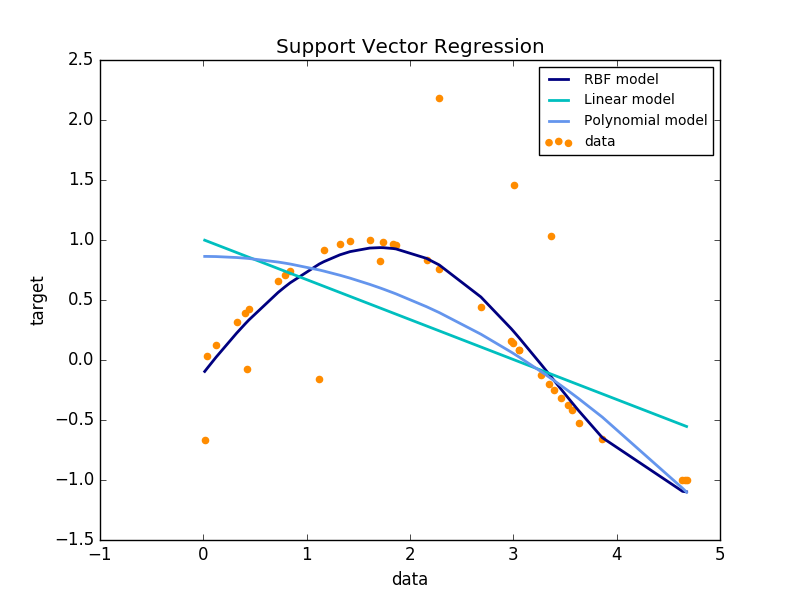
\includegraphics[height=3.5in]{figures/svr.png}
			\caption{SVR [Fuente: \href{http://scikit-learn.org/stable/auto_examples/svm/plot_svm_regression.html}{scikit learn}] }
		\end{center}
		\label{svr}
	\end{figure}
	
	\subsection{Redes Neuronales}
	\label{makereference4.3.3}
	Las redes neuronales son un algoritmo de aprendizaje supervisado de la familia de los \textbf{clasificadores}, al igual que SVR \ref{makereference4.3.2}.

	Se basan en el principio del funcionamiento de las neuronas del cuerpo humano. Cada neurona recibe varias señales y propaga, en función de estas, otro resultado al resto de la red.

	Las neuronas de estas redes, son llamadas \textbf{perceptrones}. Son unidades funcionales sin una función específica que buscan aplicar un peso a las señales recibidas y en base a ello, envía un señal a otra neurona.

	\begin{figure}[htb]
		\begin{center}
			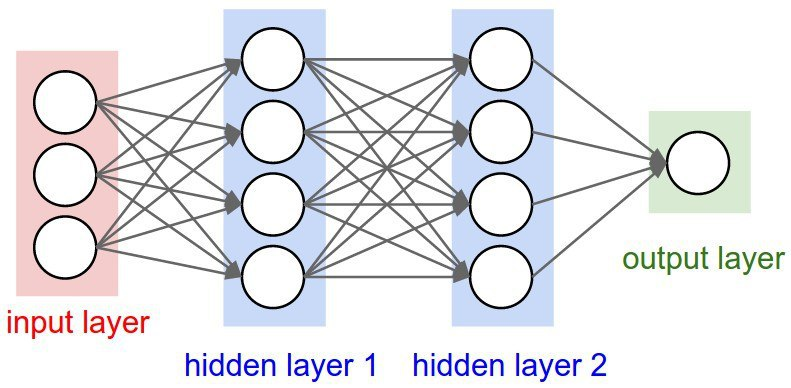
\includegraphics[width=4.5in]{figures/neural_network.jpg}
			\caption{Red neuronal [Fuente: \href{www.scikit-learn.org}{scikit-learn}]}
		\end{center}
		\label{network}
	\end{figure}

	La distribución de las neuronas se realiza en distintas capas. La primera capa ``capa de entrada'' recibe los datos de entrada. La última capa proporciona los resultados de la \textbf{clasificación}, normalmente la clase a la que pertenecen los datos de entrada.

	Las capas intermedias buscan aumentar la posibilidad de ajuste de los pesos. El ajuste de estos pesos se realiza de la siguiente forma:

	\begin{itemize}
		\item Cada neurona empieza con unos pesos aleatorios.
		\item Se introducen datos aleatorio dentro del conjunto total de entrada.
		\item La red genera un vector de datos de salida.
		\item Esta salida se compara con el resultado esperado.
		\item El \textbf{error} obtenido se propaga a la capa de neuronas anterior (\textbf{back-propagation}) y se usa para ajustar los pesos.
		\item Se continua propagando el error hacia atrás ajustando los pesos de cada capa hasta alcanzar la \textbf{capa de entrada}.
		\item Esto se repetirá con diferentes datos de entrenamiento.
 	\end{itemize}

	Es tarea del desarrollador la elección del número de capas y de neuronas en cada capa.

\section{Método de estudio}
\label{makereference4.4}
	\subsection{Grid Search}

	\begin{figure}[htb]
		\begin{center}
			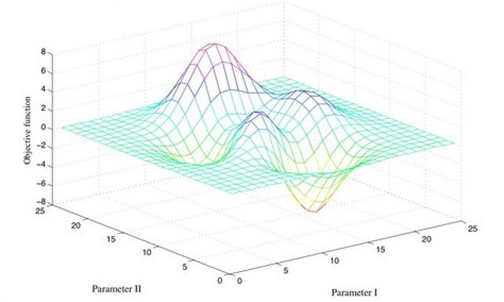
\includegraphics[width=4in]{figures/grid_search.png}
			\caption{Grid Search [Fuente: \href{www.scikit-learn.org}{scikit-learn}]}
		\end{center}
		\label{grid}
	\end{figure}

	Para optimizar la elección del modelo predictivo y sus parámetros, necesitamos estudiar el comportamiento que tiene un modelo con todos sus posibles valores en cada parámetro, teniendo así la certeza de que elegimos la mejor configuración.

	Esta es una tarea que no se puede llevar a cabo debido a su complejidad computacional, por lo que existen distintas maneras de abordar el problema. En respuesta a esto, surgen métodos de análisis más optimos, entre ellos encontramos \textbf{Grid Search}.

	\textbf{Grid Search} es un método de estudio ya implementado al que se le especifica los algoritmos a estudiar y rangos para los distintos parámetros de cada uno. 

	Este método observa qué muestra del rango es la que obtiene un ``mejor resultado'' y vuelve a realizar el estudio ``haciendo zoom'' con centro en esta muestra.

	Para calcular el mejor resultado se utiliza una técnica llamada \textbf{``K-Fold Cross-Validation''}. Esta técnica divide los datos en ``k'' conjuntos. Uno de ellos es utilizado como datos de prueba y el resto como datos de entrenamiento. Se realiza un proceso de validación y se repite k veces con cada uno de los posibles subconjuntos. Ver figura \ref{cross}.

	Al realizar este proceso de validación con datos conocidos, puede conocer la precisión o ``accuracy'' que es capaz de obtener un modelo predictivo.

	Una vez realizado el estudio con los distintos modelos y parámetros se puede observar cual es la mejor configuración para nuestros datos.

	\begin{figure}[htb]
		\begin{center}
			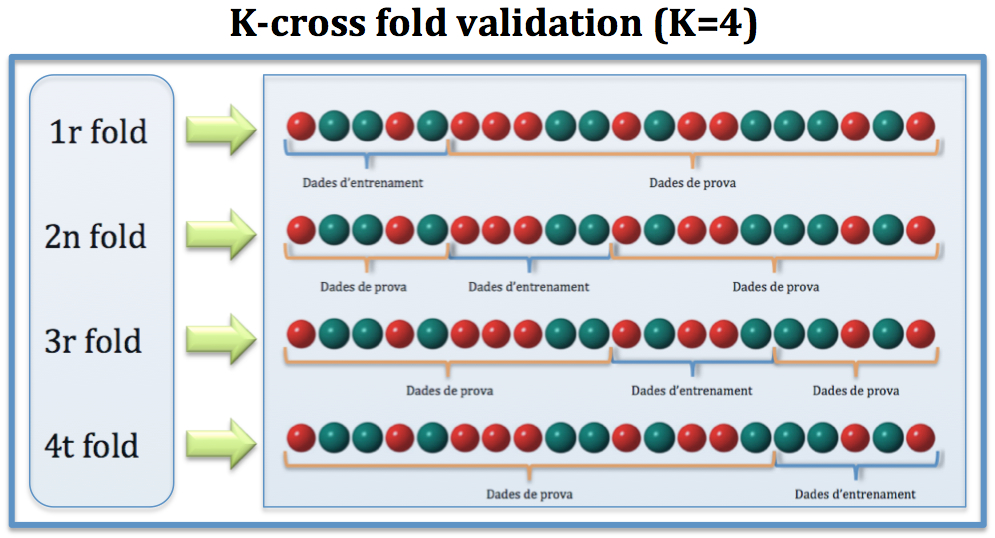
\includegraphics[width=4.5in]{figures/Cross-Validation.jpg}
			\caption{Validación cruzada [Fuente: \href{www.scikit-learn.org}{scikit-learn}]}
		\end{center}
		\label{cross}
	\end{figure}
	
	Existen otros métodos de exploración del modelo predictivo como por ejemplo \textbf{Randomized Parameter Optimization}, que realiza el estudio probando con configuraciones aleatorias.

	\subsection{Sistema de entrenamiento}
	
	\begin{figure}[htb]
		\begin{center}
			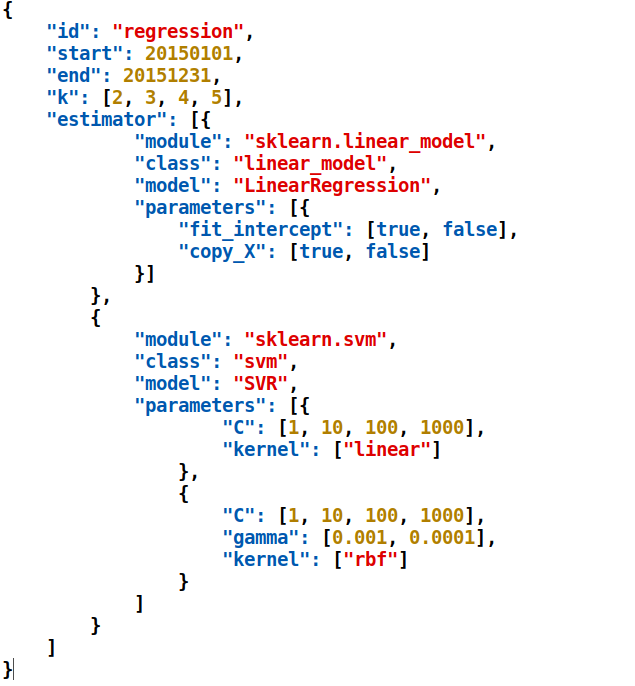
\includegraphics[height=5.5in]{figures/json_conf.png}
			\caption{Ejemplo JSON de prueba}
		\end{center}
		\label{json}
	\end{figure}

	Para llevar a cabo la implementación de Grid Search, hemos utilizado las funciones proporcionadas por \textbf{scikit-learn} (\cite{ARP:Scikit:2017}).
	Esta librería ofrece una implementación de Grid Search a través de una función que nos permite abstraer el algoritmo de los modelos predictivos.

	Hemos desarrollado distintas baterías de pruebas a través de ficheros en formato \href{www.json.org/json-es.html}{JSON} (JavaScript Object Notation) que definen los distintos modelos y parametros que debe explorar Grid Search.
	Estas baterias de prueba son procesadas por un algoritmo encargado de instanciar los distintos modelos y suministrárselos a Grid Search. Ver figura \ref{json}.

	Los resultados obtenidos de cada prueba son almacenados en archivos con formato CSV para su posterior análisis. Ver figura \ref{csv}.	

	\begin{figure}[htb]
		\begin{center}
			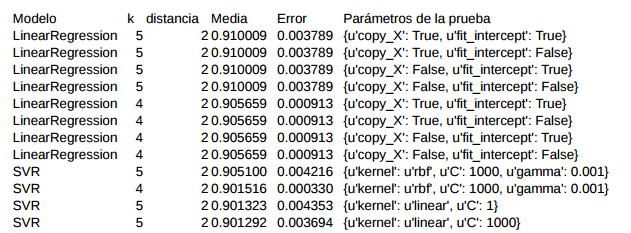
\includegraphics[width=17cm]{figures/resultados_grid_csv.png}
			\caption{Ejemplo de resultados Grid Search}
		\end{center}
		\label{csv}
	\end{figure}

	Las columnas de los resultados son:
	\begin{itemize}
		\item \textbf{Modelo:} Nombre del algoritmo usado.
		\item \textbf{k:} Número de muestras anteriores utilizadas para predecir.
		\item \textbf{Distancia:} Número de muestras posteriores sobre la que se quiere encontrar la predicción.
		\item \textbf{Media:} Valor entre 0 y 1 que indica la precisión de la predicción.
		\item \textbf{Error:} Valor entre 0 y 1 que indica la desviación típica de esta predicción.
		\item \textbf{Parámetros de la prueba:} Configuración de los posibles valores con los que se han obtenido la media y el error.
	\end{itemize}

	Una vez elegido el modelo predictivo y su configuración, podemos volver a entrenar el sistema guardando el resultado de este entrenamiento. De esta forma, en el momento de la predicción no necesitaremos volver a entrenar porque los parámetros del modelo están \textbf{ajustados}.

\section{Descripción de las librerías usadas}
\label{makereference4.5}
	\subsection{Scikit-learn}
	\label{makereference4.5.1}
	Scikit-learn es una biblioteca de aprendizaje de software libre para el lenguaje de programación Python. Cuenta con varios algoritmos de clasificación, regresión y agrupación, incluyendo máquinas de vector de apoyo, bosques aleatorios y aumento de gradiente, y está diseñado para interoperar con las bibliotecas numéricas y científicas Python NumPy y SciPy. (\cite{ARP:Scikit:2017})
	
	\subsection{NumPy}
	\label{makereference4.5.2}
	NumPy es una extensión de Python, que le agrega mayor soporte para vectores y matrices, constituyendo una biblioteca de funciones matemáticas de alto nivel para operar con esos vectores o matrices. (\cite{ARP:Numpy:2017})